\subsection{Ribbon-10L histogram of interpolated points}

\begin{table}[ht]
	\begin{center}
		\begin{tabular}[top]{ p{16.0 cm} }
			\frame{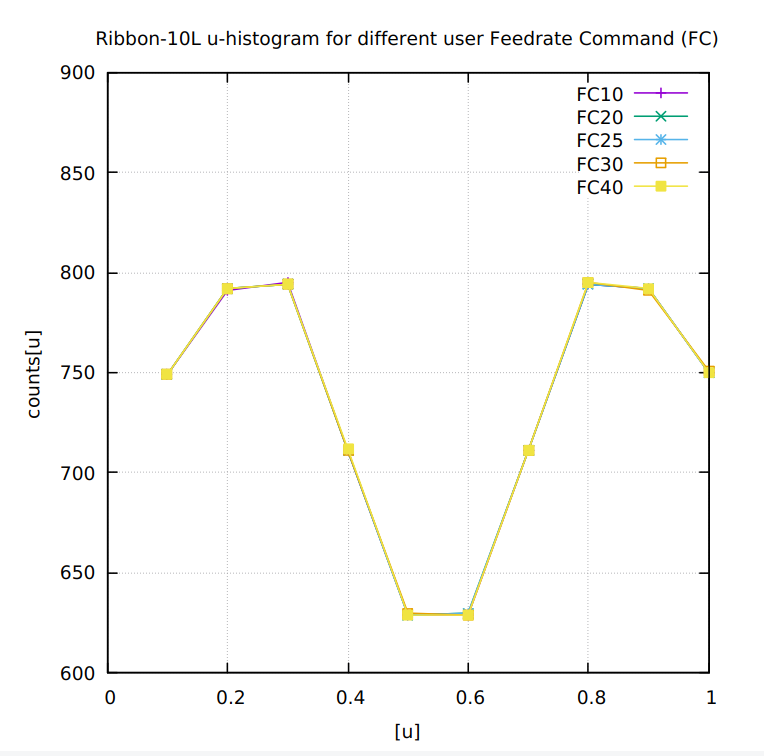
\includegraphics[width=0.95\textwidth]{./07-images/img-Ch54/Img-09-Ribbon-10L-u-histogram.png}}\\
		\end{tabular}
		\caption{Ribbon-10L histogram of interpolated points}		
		\label{table:Ribbon-10L histogram of interpolated points}
	\end{center}
\end{table} 
